\documentclass[letterpaper,11pt]{./templates/texMemo} % Set the paper size (letterpaper, a4paper, etc) and font size (10pt, 11pt or 12pt)

\usepackage{graphicx}
\graphicspath{ {../img/} }
\usepackage[parfill]{parskip} % Adds spacing between paragraphs
\setlength{\parindent}{0pt} % Indent paragraphs

%----------------------------------------------------------------------------------------
%   MEMO INFORMATION
%----------------------------------------------------------------------------------------

\memoto{Industrial Consultant} % Recipient(s)

% Setup of the document
\memosubject{Project Brief}
\memofrom{Team 14 - Daniel DeHoog, T.J. DeVries,
    Paul Griffioen, Ryan Siekman}

\memodate{October 19, 2015}

% Now the writing of the document can begin
\begin{document}

\maketitle 

\section{Team Members}

% Include the team members
\centerline{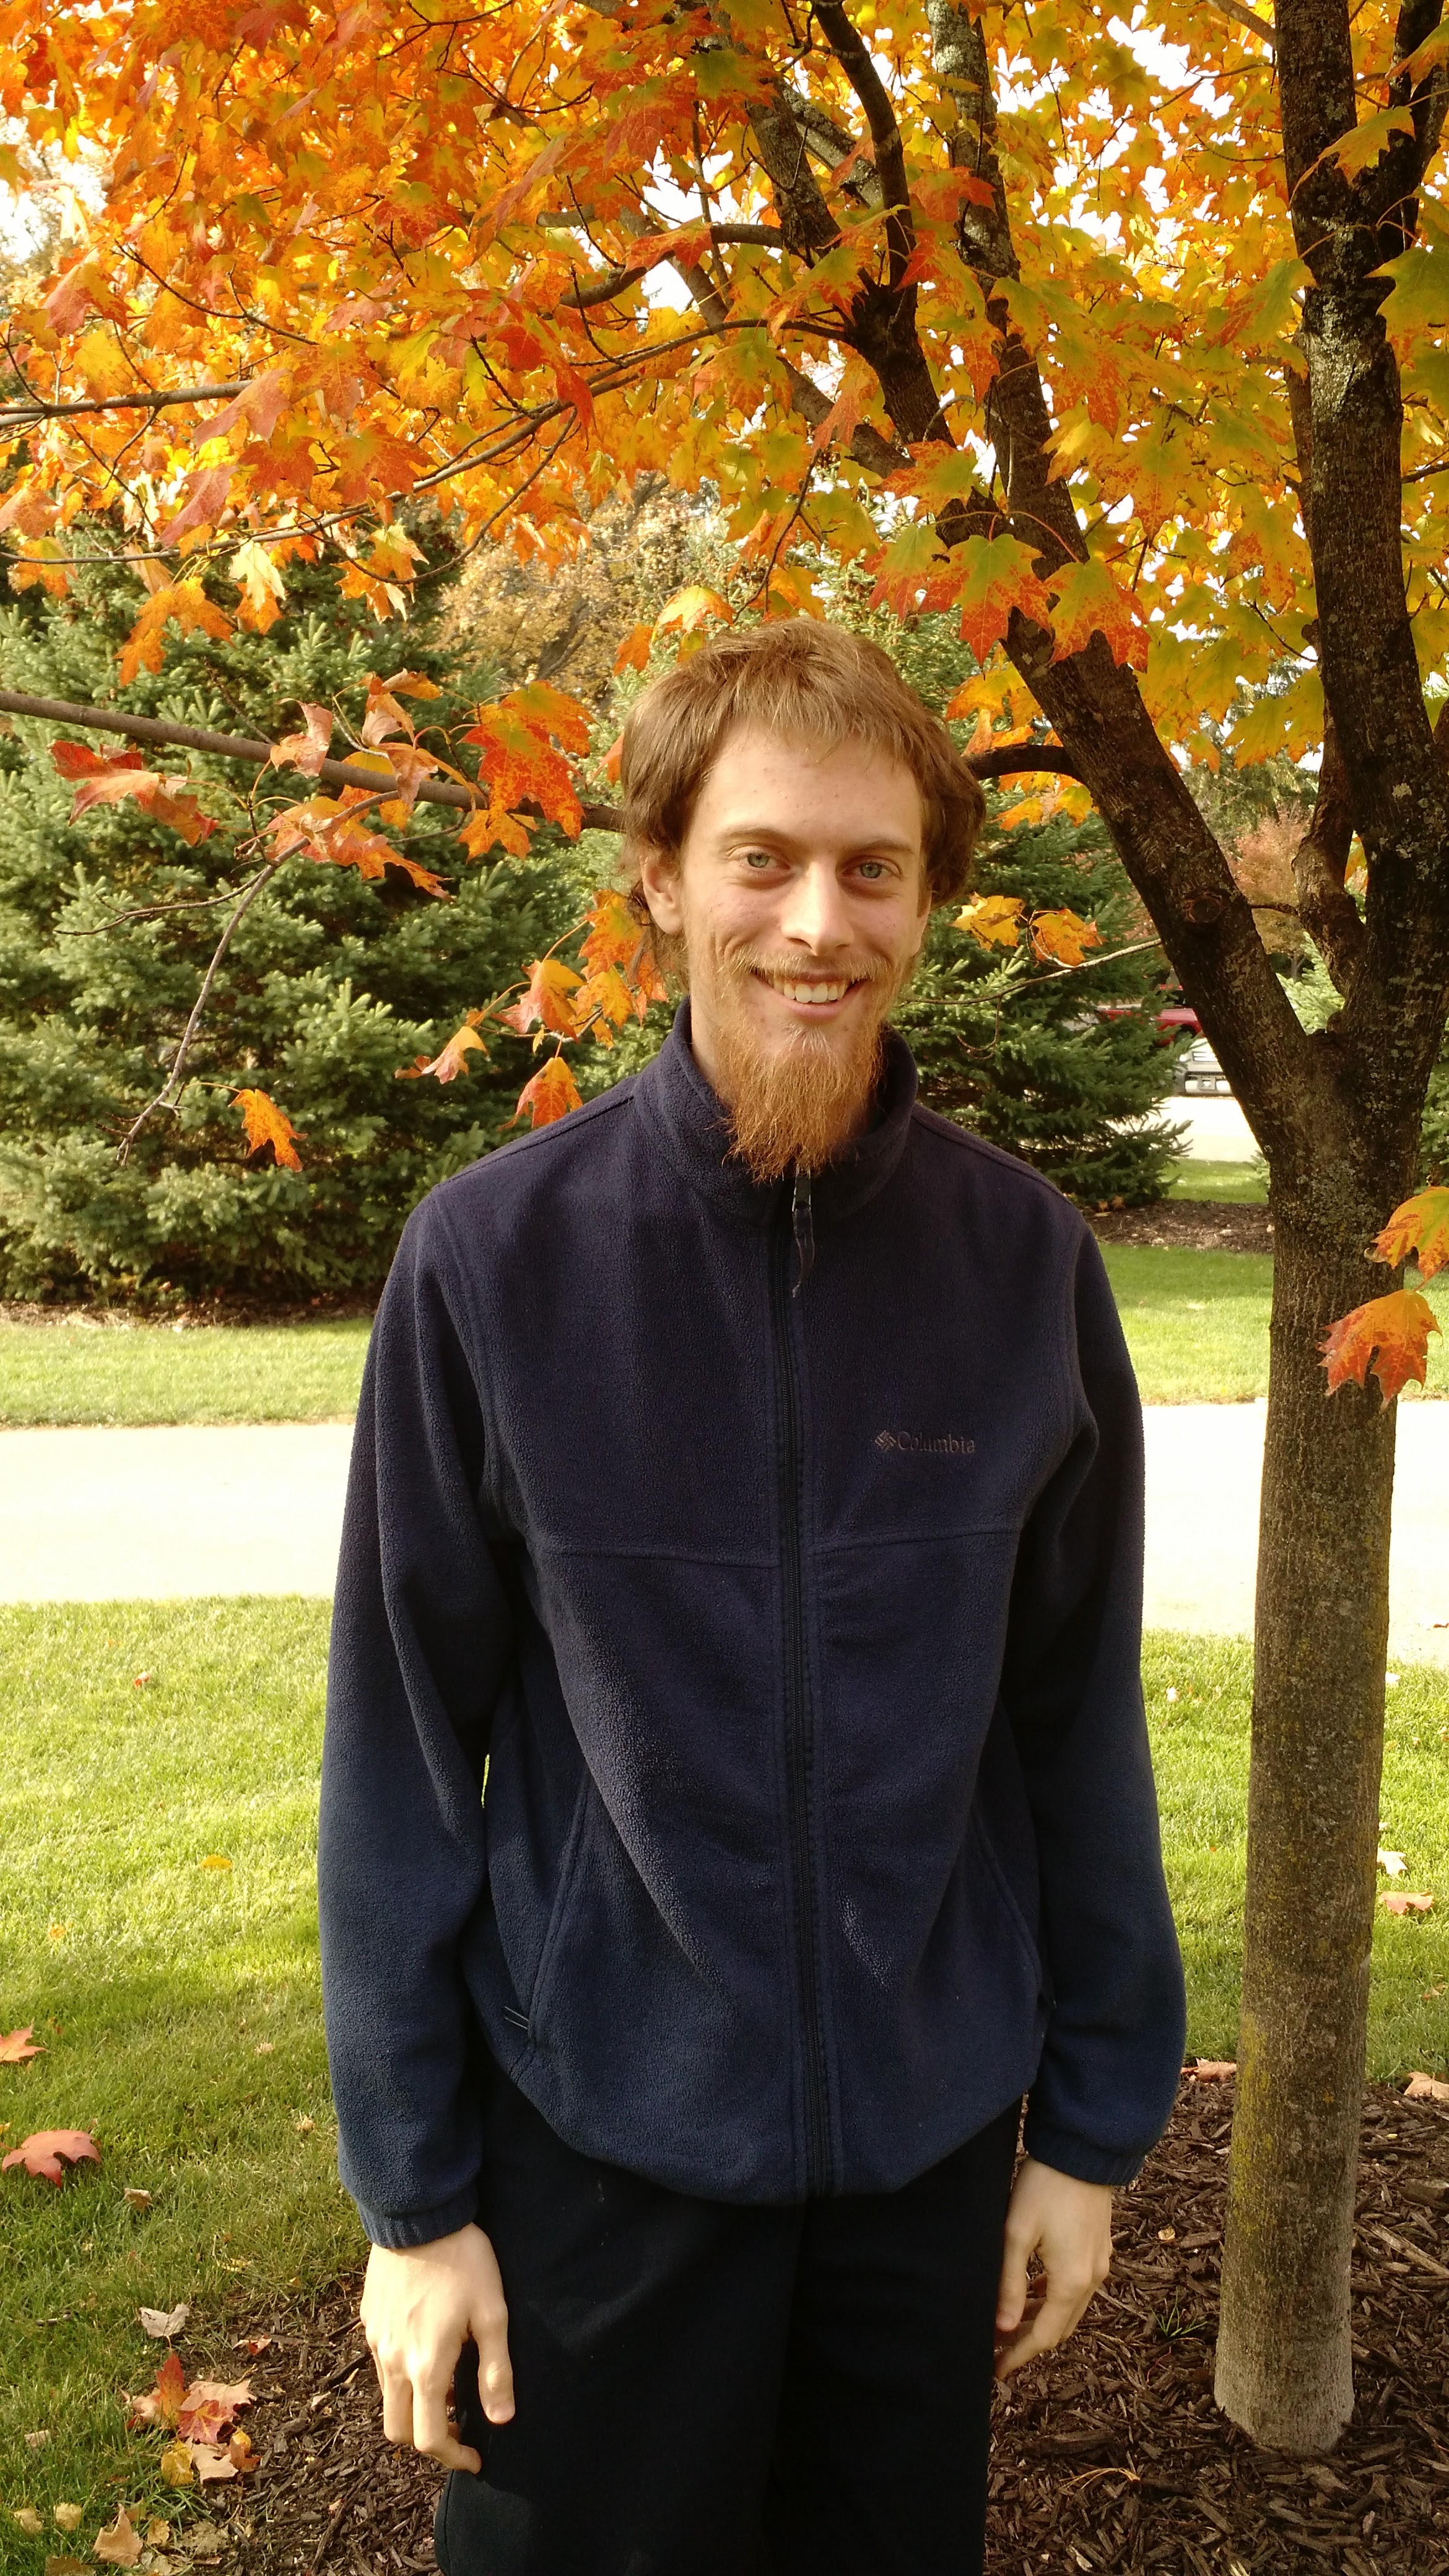
\includegraphics[width=0.25\textwidth]{dan.jpg} 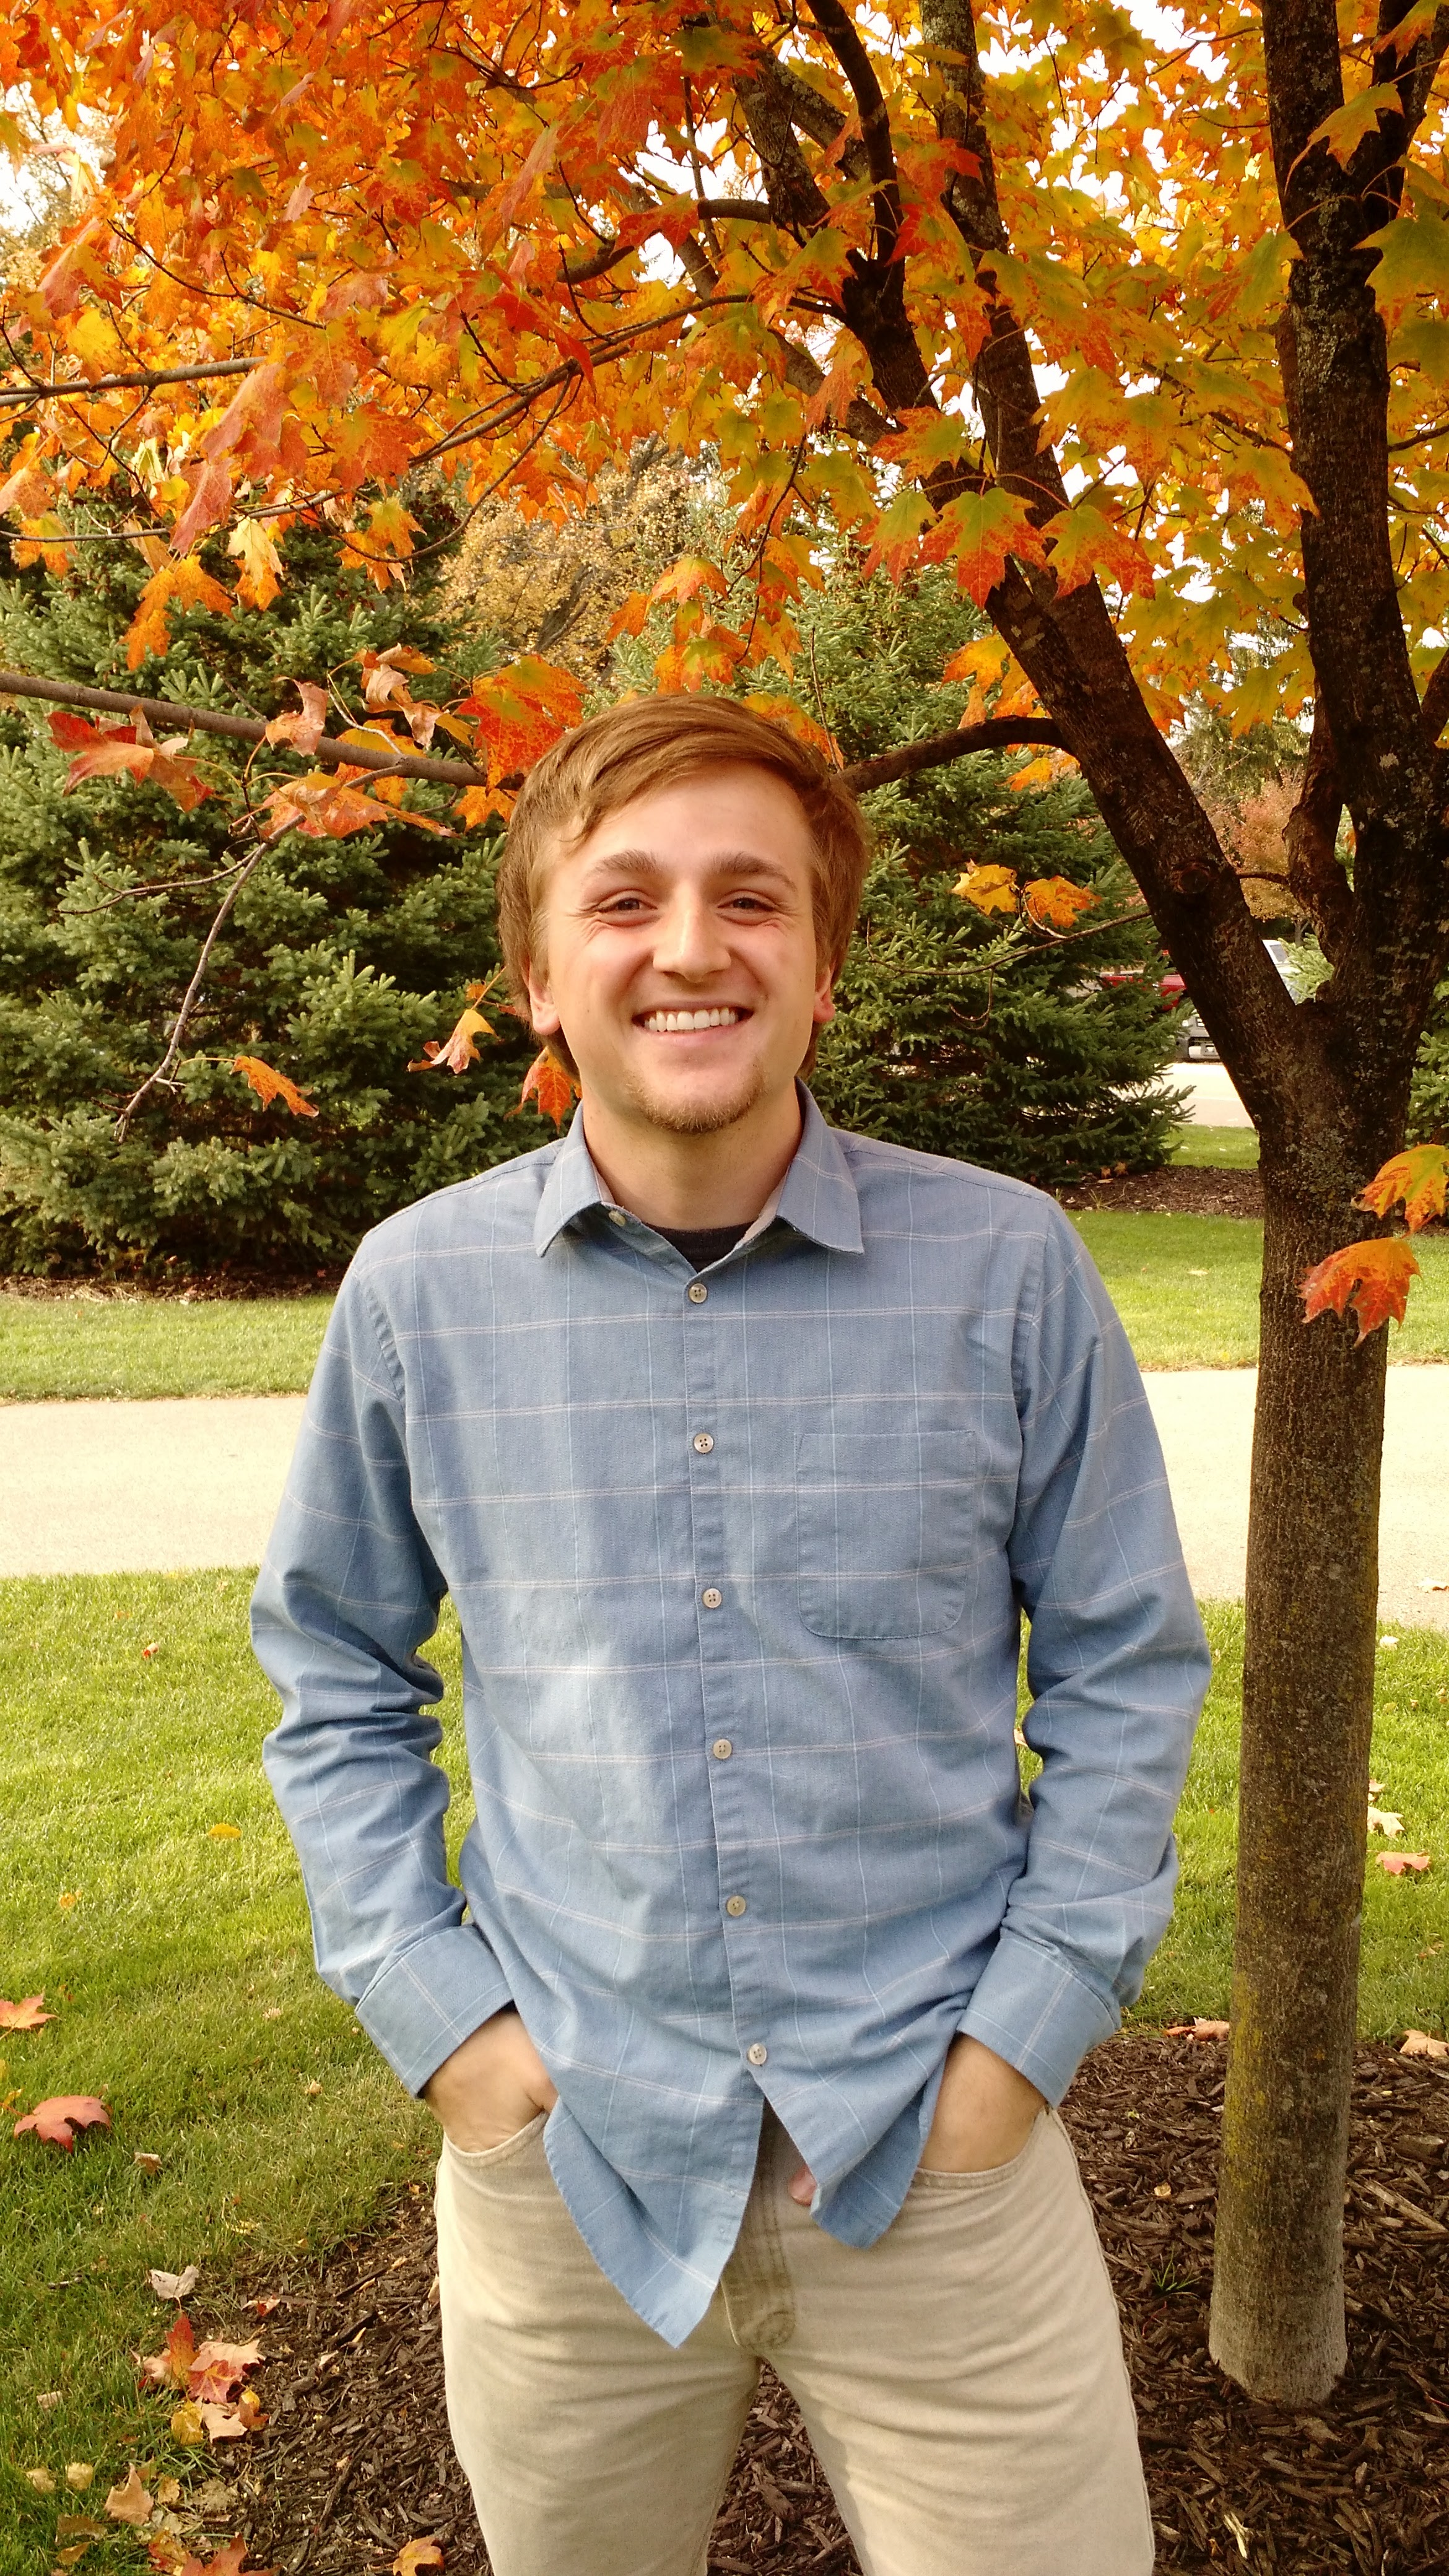
\includegraphics[width=0.25\textwidth]{tj.jpg} 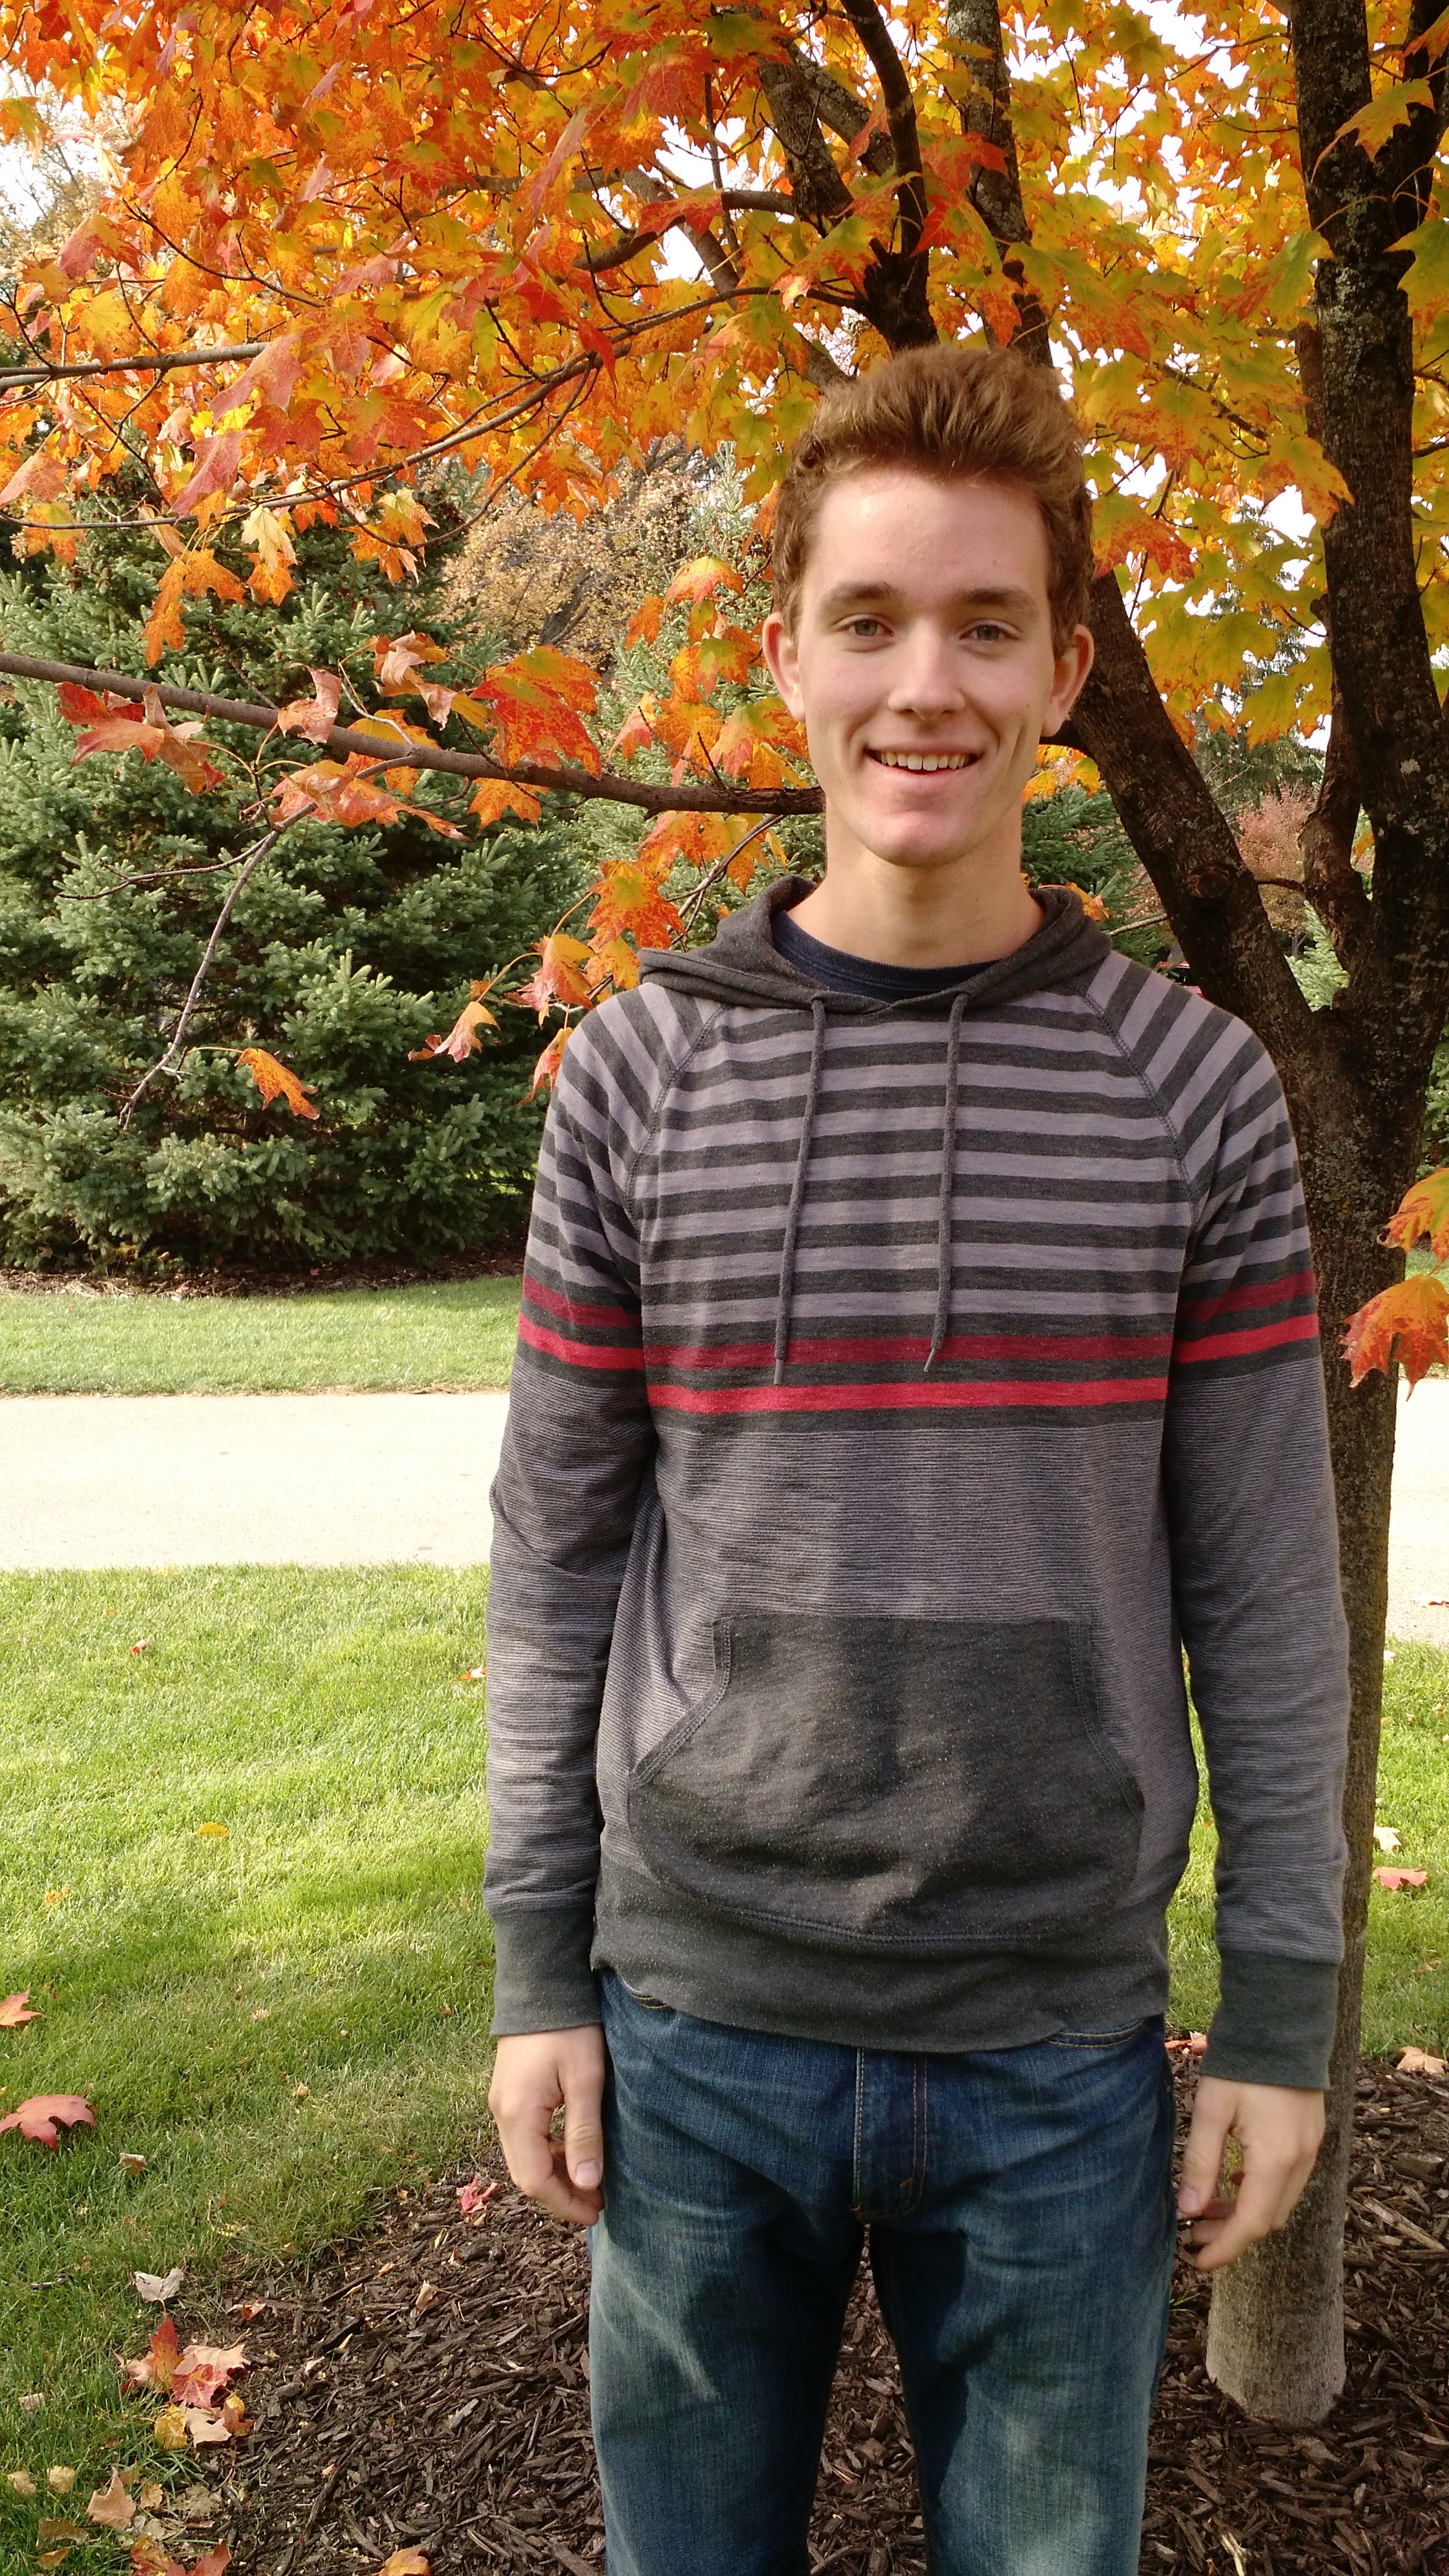
\includegraphics[width=0.25\textwidth]{paul.jpg} 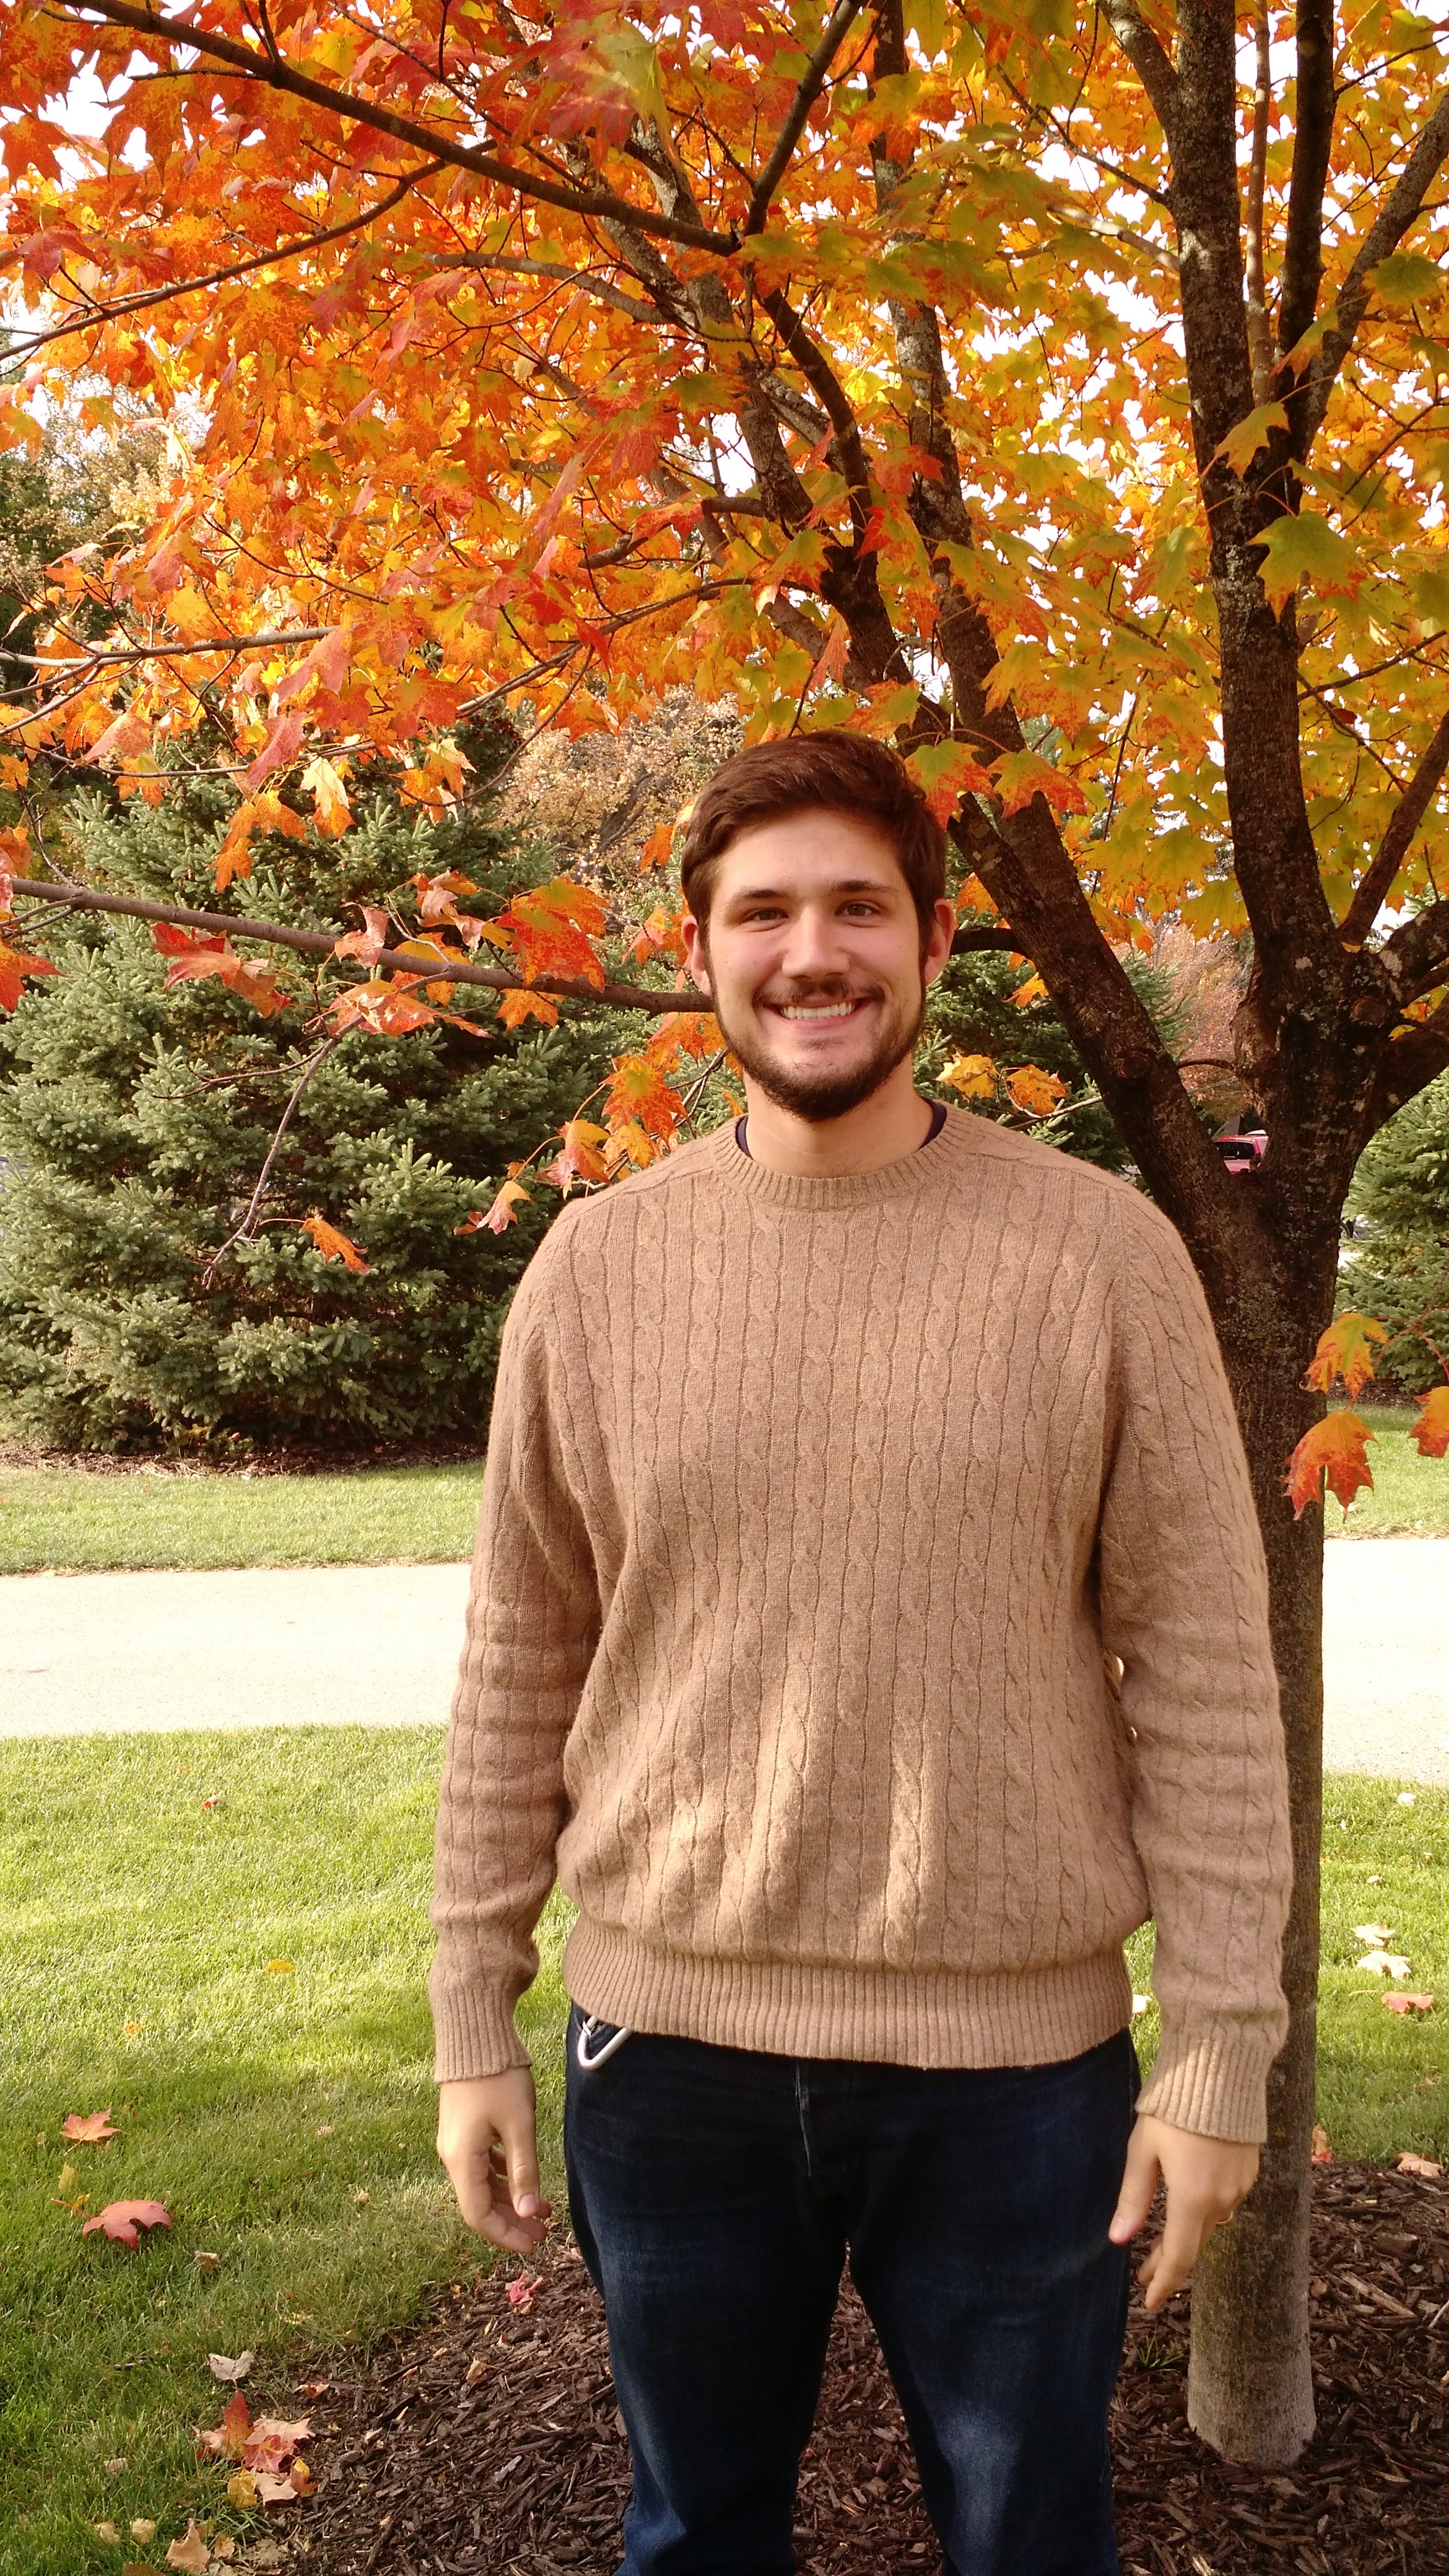
\includegraphics[width=0.25\textwidth]{ryan.jpg}}
\centerline{Daniel DeHoog, TJ DeVries, Paul Griffioen, Ryan Siekman}

\section{Project Description}

Create a system that will allow people, both clients and administrators, to interact with gyms in a modern and smart way. This system will allow users to view what machines are currently open, and it will also allow users to reserve systems for personal use. The system will also provide gym administrators with the ability to understand more clearly what machines get used, along with how often and when they are used.

\section{Project Requirements}

The following subsections list the project requirements, which are divided into system requirements and hardware requirements. Necessary requirements are listed as is, whereas optional requirements are presented in brackets.

\subsection{System Requirements}

    \begin{itemize}
    \item{\textbf{Generic}}
    \begin{itemize}
        \item{Ability to install the system in a typical existing gym}
        \item{Transferable - ability to transfer sensors and displays from one type of machine/equipment to another}
        \item{Ability to install each sensor and each display on (most) any type of stationary equipment}
        \item{[Ability to install sensors on free weights, weight sets, and other moving equipment]}
    \end{itemize}

    \item{\textbf{General}}
    \begin{itemize}
        \item{Ability to run continuously for 24 hours without crashing}
        \item{Price is small enough that existing gyms would be willing to invest in buying it}
        \item{Ability for gyms to only use parts of the system if desired}
        \item{Ability to add or remove parts after initial setup and installation}
    \end{itemize}

    \item{\textbf{Accessibility}}
    \begin{itemize}
        \item{Data should be accessible via a web interface (mobile device and personal computer)}
        \item{Detailed data about equipment use should be accessible for gym managers}
        \item{[Fitness data should be available for personal use]}
    \end{itemize}

    \item{\textbf{User-Friendly}}
    \begin{itemize}
        \item{Sensors should not impede use of machinery or weights}
        \item{Web interface and mobile application should be simple and easy to use}
    \end{itemize}

    \item{\textbf{Reservation System}}
    \begin{itemize}
        \item{Organized according to machine, user, and time}
        \item{Implement rules about making reservations and canceling them to protect against system abusers}
        \item{Reservation information for a specific machine should appear on that machine's display}
        \begin{itemize}
            \item{Allow user to interact with the display to edit the reservation}
        \end{itemize}
        \item{No power supply required for reservation display or sensors}
        \item{[Bulk reservations (over multiple periods of time)]}
        \item{[Electronic calendar integration]}
    \end{itemize}

    \item{\textbf{Real-Time Updates}}
    \begin{itemize}
        \item{Real-time updates of which machines are currently being used}
        \begin{itemize}
            \item{Each update occurs within one minute}
        \end{itemize}
        \item{Based on data acquired from sensors, not data used from reservation system}
    \end{itemize}

    \item{\textbf{Central Management}}
    \begin{itemize}
        \item{Smart hub, located within the gym, must collect data from the sensors and communicate data to the displays}
        \item{Data will be collated by a central server}
        \begin{itemize}
            \item{Central server will manage the reservation system, web interface, and mobile application}
        \end{itemize}
        \item{[Smart hub will cache daily schedules for sending to the displays in case internet connection is lost]}
    \end{itemize}
    \end{itemize}

\subsection{Hardware Requirements}

    \begin{itemize}
    \item{\textbf{Sensors}}
    \begin{itemize}
        \item{Used to determine whether or not a machine is in use}
        \item{Must be movement sensors (accelerometer, gyroscope, or magnetometer) on a single board}
        \item{Long battery life, on the order of years}
        \item{Small size (less than 5 in$^2$)}
        \item{Possess network capabilities with the ability to form a mesh network, where the sensors can communicate with and pass data to one another}
        \item{Ability to make strong yet removable physical connections to each machine}
    \end{itemize}
    
    \item{\textbf{Display Interfaces}}
    \begin{itemize}
        \item{Used to display machine reservations}
        \item{Long battery life, on the order of months}
        \item{Display information, such as a name and reservation time, in a user-friendly manner}
        \item{Ability to handle sweat that may fall on the display}
        \item{Possess network capabilities with the ability to form a mesh network, where the displays can communicate with and pass data to one another}
        \item{Display must be compatible with the mesh network}
        \item{Relatively small (approx. 2 in by 3 in) with at least 2 push buttons and 1 LED for making reservations}
    \end{itemize}
    
    \item{\textbf{Hub}}
    \begin{itemize}
        \item{A small yet powerful computer (raspberry pi) placed within the gym}
        \item{Capable of running multiple operating systems (Linux and Windows)}
        \item{Ethernet connection for reliable internet connection}
        \item{Ability to communicate with the mesh network of sensors and displays (wifi, zigbee, bluetooth)}
        \item{[Ability to turn on and off sensors and displays to save energy]}
    \end{itemize}
    
    \item{\textbf{Server}}
    \begin{itemize}
        \item{A reliable computer with the ability to communicate with the hub}
        \item{Host the website and mobile application that users employ for reservations and seeing which machines are currently in use}
        \item{Store the database of information for reservations and data collected from the sensors}
    \end{itemize}
    \end{itemize}

\section{Current Project Status}		

Since we have determined the project requirements, the main tasks our team is currently working on are determining alternative designs that satisfy the requirements and working on the PPFS. In addition, we are determining what tools we want to use to facilitate project management and collaboration during the project.

The alternatives we are attempting to determine include what hardware we want to use for our sensors and for the display interfaces, which includes both the display itself and the board used for wireless communication. The difficulty in this task is finding hardware that possesses both low power, is capable of communicating in a mesh network, and is compatible with the other hardware. For the hub, we have decided to use a Raspberry Pi coupled with wireless modules to communicate with the display interfaces and the sensors.

For project management, we are using Microsoft Project coupled with a Google spreadsheet to allow us to collaborate when managing the project. We are also using a distributed version control system "Git" to facilitate collaboration on design files and reports while giving us more control to manage the files over time.

\end{document}
